
\chapter{Enabling Technologies}
\label{chap:enabling_technologies}
\begin{chapterintro}
This chapter introduces which technologies have made possible this project. First of all there must be an engine to build the game application, this is Unity game engine, explained in section \ref{sec:unity}. Secondly, Unity integrates third part software as plugins to facilitate development through its Asset Store, this components are detailed in section \ref{sec:assetstore}. Finally, there should be a tool to manage application metrics and information after its deployment, this is done by Flurry Analytics, explained in section \ref{sec:flurry}.
\end{chapterintro}

\cleardoublepage
\section{Unity3D game engine}
\label{sec:unity}
Today’s game creators rely on game engines to develop the main pieces of software for their games. A game engine simplifies the task of the programmers by offering convenient abstractions for the hardware and operating systems on top of which the game runs.~\cite{messaoudi2015dis}

Gamers play on so many different types of devices which have lots of differences regarding their hardware and software resources. One of the main purposes of a game engine is to make this development easier avoiding building one application for each device we want to be compatible with.

Unity3D game engine is an integrated development tool for producing other interactive contents such as video game, architectural visualization, real-time 3D animation. Its editor runs on Window, Mac OS X, so it could make games as the platforms of Window, Mac, Wii, iPad, and iPhone. It could also produce web browser game that uses unity web player plug-in. This is a similar form of flash, and it is designed so that flash user could easily adapt even with cross domain security policy and scripting.

The functions that Unity3D supports autonomously are very abundant. In fact, all game developments are possible such as shader, physics engine, network, terrain manipulation, audio, video, and animation, and it considered so that the revision is possible to the taste of user according to the need. Unity3D that produces based on Java script and C\# can apply and manage after producing the desired functions with script, not producing all of the programing at once. GUI composed on screen helps the first-time developer to approach easily, and the script and program that programer made with simple mouse drag.~\cite{kim2014dev}

\begin{figure}[h]
\centering

\includegraphics[width=200pt]{graphics/enabling-tech/unity_logo.png}
\caption{Unity3D logo}
\label{fig:unity_logo}
\end{figure}

Unity3D is a flexible and high-performance development platform used to make creative and intelligent interactive 3D and 2D experiences. The "author once, deploy everywhere" capability ensures developers can publish to all of the most popular platforms. Unity Technologies boasts a thriving community of over 2 million developers including large publishers, indie studios, students and hobbyists. To remain at the forefront of innovation, Unity Technologies tirelessly re-invests in its award-winning 3D development tools and its democratization initiatives, such as the Asset Store digital content marketplace and Unity Games publishing and distribution division.~\cite{unitypress1}

We will detail Unity3D components and how those components will be integrated in the application development in the following subsections. Frstly we will detail Unity3D principal features in \ref{subsec:unityfeatures}, secondly in \ref{subsec:unityinterface} we are going to explain Unity3D interface from where we create our game and finally in \ref{subsec:unitycomponents} we are going to explain all the components seen on that interface:

\subsection{Unity3D features}
\label{subsec:unityfeatures}
The latest update, Unity 4.6, was released in August, 2012. It currently supports development for iOS, Android, Windows, OS X, Linux, web browsers, Flash, PlayStation 3, Xbox 360, and Wii U.~\cite{unitypress2} The game engine can be downloaded from their website in two different versions: Unity and Unity Pro. Between its features we can point highlight the following:
\begin{itemize}
\item \textit{Rendering}, The graphics engine uses Direct3D (Windows), OpenGL (Mac, Windows,
Linux), OpenGL ES (Android, iOS), and proprietary APIs (Wii). There is support for bump mapping, reflection mapping, parallax mapping, screen space ambient occlusion (SSAO), dynamic shadows using shadow maps, render-to-texture and full-screen post-processing effects.
Unity supports art assets and file formats from 3ds Max, Maya, Softimage, Blender, Modo, ZBrush, Cinema 4D, Cheetah3D, Adobe Photoshop, Adobe Fireworks and Allegorithmic Substance. These assets can be added to the game project, and managed through Unity's graphical user interface.~\cite{unitypress3}
The ShaderLab language is used for shaders, supporting both declarative "programming" of the fixed-function pipeline and shader programs written in GLSL or Cg. A shader can include multiple variants and a declarative fallback specification, allowing Unity to detect the best variant for the current video card, and if none are compatible, fall back to an alternative shader that may sacrifice features for performance.~\cite{unitypress4}
\item \textit{Scripting}, The game engine's scripting is built on Mono, the open-source implementation
of the .NET Framework. Programmers can use UnityScript (a custom language with ECMAScript-inspired syntax), C\# or Boo (which has a Python-inspired syntax).~\cite{unitypress5} Starting with the 3.0 release, Unity ships with a customized version of MonoDevelop for debugging scripts.~\cite{unitypress6}
\item \textit{Asset Tracking}, Unity also includes the Unity Asset Server, a version control solution for the developer's game assets and scripts. It uses PostgreSQL as a backend, an audio system built on the FMOD library (with ability to playback Ogg Vorbis compressed audio), video playback using the Theora codec, a terrain and vegetation engine (which supports tree billboarding, Occlusion Culling with Umbra), built-in lightmapping and global illumination with Beast, multiplayer networking using RakNet, and built-in pathfinding navigation meshes.~\cite{unitypress7}
\item \textit{Platforms}, Unity supports deployment to multiple platforms. Within a project, developers
have control over delivery to mobile devices, web browsers, desktops, and consoles.~\cite{unitypress2}
Unity also allows specification of texture compression and resolution settings for each platform the game supports.~\cite{unitypress2}
Currently supported platforms include Windows, Linux, Mac, Android, iOS, Unity Web Player, Adobe Flash, PlayStation 3, Xbox 360, and Wii. Although not officially confirmed, Unity also supports the PlayStation Vita as can be seen on the game Escape Plan. Upcoming platforms include BlackBerry 10, Wii U, Windows 8, and Windows Phone 8.
\item \textit{Asset Store}, Launched in November 2010, the Unity Asset Store is a resource available
within the Unity editor. The store consists of a collection of over 4,400 asset packages, including 3D models, textures and materials, particle systems, music and sound effects, tutorials and projects, scripting packages, editor extensions and online services. We will detail this feature in section \ref{sec:assetstore}. The store also contains many extensions, tools and asset packages such as the package 2D Toolkit, which provides an efficient \& flexible 2D sprite, collider set-up, text, tilemap and UI system integrating seamlessly into the Unity environment.
\item \textit{Versions}, The first version of Unity was launched at Apple’s Worldwide Developers Conference in 2005. It was built to function and build projects on Mac computers and garnered enough success to continue development of the engine and tools for other platforms.[2] Unity 3 was released in September 2010 and focused on introducing more of the tools that high-end studios have at their disposal. This allowed the company to capture the interest of bigger developers while providing independent and smaller teams with a game engine in one affordable package. The latest version of Unity, Unity 4.6, was released in August 2014, and includes features such as New UI System: Design UIs for your game or application using Unity's powerful new component based UI framework and visual tools and an extensible event messaging system.
\end{itemize}

\subsection{Unity3D interface}
\label{subsec:unityinterface}
When we create a project, the first thing we see is Unity3D interface. This interface can be easily customized so that it would fits developer needs. In figure \ref{fig:unity_interface_general} we can see the interface that we have to used during the game development process.

\begin{figure}[h]
\centering
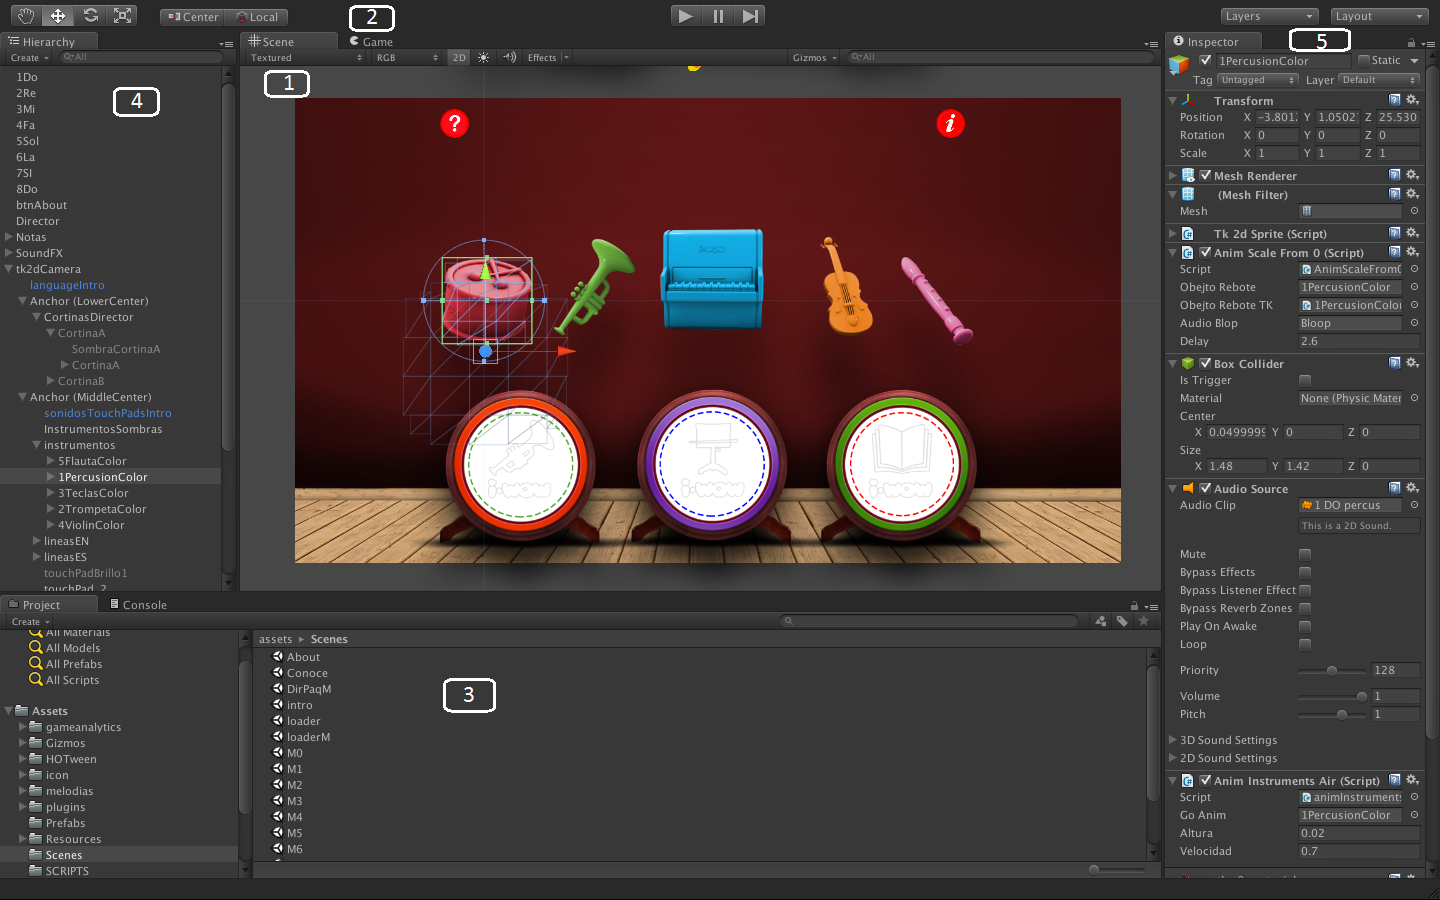
\includegraphics[width=450pt]{graphics/enabling-tech/unity_interface_general.png}
\caption{Unity3D interface}
\label{fig:unity_interface_general}
\end{figure}

\subsection{Unity3D components}
\label{subsec:unitycomponents}

\section{Unity Asset Store}
\label{sec:assetstore}


\section{Flurry analytics}
\label{sec:flurry}
